%! Author = zhiweizhang
%! Date = 12.06.25

% Preamble
\begin{figure}[ht]
    \centering
    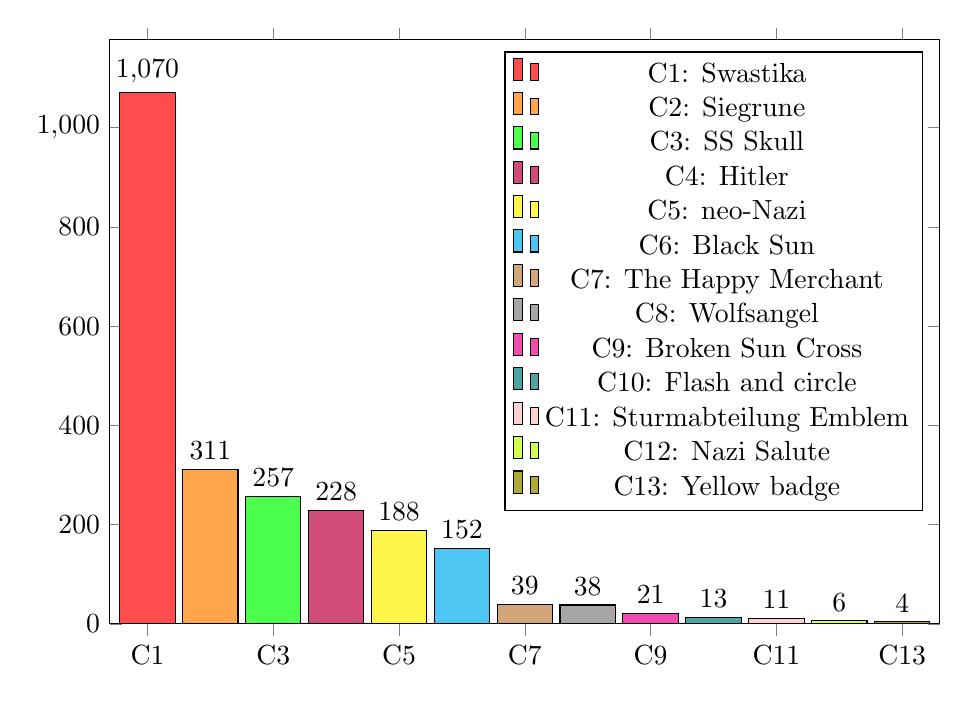
\begin{tikzpicture}
      \begin{axis}[
        ybar,
        bar width=20pt,
        width=\textwidth,
        height=9cm,
        symbolic x coords={C1,C2,C3,C4,C5,C6,C7,C8,C9,C10,C11,C12,C13},
        enlarge x limits=.05,
        nodes near coords,
        nodes near coords align={vertical},
        bar shift=0pt,
        ymin=0,
      ]

            % bars with color coding
            \addplot[fill=red!70] coordinates {(C1,1070)};
            \addplot[fill=orange!70] coordinates {(C2,311)};
            \addplot[fill=green!70] coordinates {(C3,257)};
            \addplot[fill=purple!70] coordinates {(C4,228)};
            \addplot[fill=yellow!70] coordinates {(C5,188)};
            \addplot[fill=cyan!70] coordinates {(C6,152)};
            \addplot[fill=brown!70] coordinates {(C7,39)};
            \addplot[fill=gray!70] coordinates {(C8,38)};
            \addplot[fill=magenta!70] coordinates {(C9,21)};
            \addplot[fill=teal!70] coordinates {(C10,13)};
            \addplot[fill=pink!70] coordinates {(C11,11)};
            \addplot[fill=lime!70] coordinates {(C12,6)};
            \addplot[fill=olive!70] coordinates {(C13,4)};
        \legend{
            C1: Swastika,
            C2: Siegrune,
            C3: SS Skull,
            C4: Hitler,
            C5: neo-Nazi,
            C6: Black Sun,
            C7: The Happy Merchant,
            C8: Wolfsangel,
            C9: Broken Sun Cross,
            C10: Flash and circle,
            C11: Sturmabteilung Emblem,
            C12: Nazi Salute,
            C13: Yellow badge
        }
        \end{axis}
    \end{tikzpicture}
    \caption{Dataset distribution of the multi-class classification task.}
    \label{fig:multi-class-dataset-distribution}
\end{figure}
